\documentclass[12pt]{article}

\usepackage[english]{babel}
\usepackage[utf8x]{inputenc}
\usepackage[T1]{fontenc}
\usepackage{float}
\usepackage[sc,osf]{mathpazo}  
\linespread{1.025}
\usepackage{fancyvrb}
\usepackage[a4paper,top=3cm,bottom=2cm,left=2cm,right=2cm,marginparwidth=2cm]{geometry}
\usepackage{amsmath}
\usepackage{graphicx}
\usepackage[colorinlistoftodos]{todonotes}
\usepackage{enumitem}
\usepackage{listings}
\usepackage{authblk}
\usepackage{fancyhdr}
\usepackage{parskip}
\usepackage{fancyhdr}
\usepackage{vmargin}
\setpapersize{A4}
\setmarginsrb{25mm}{25mm}{25mm}{25mm}{0pt}{0mm}{0pt}{0mm}
\definecolor{dkgreen}{rgb}{0,0.6,0}
\definecolor{gray}{rgb}{0.5,0.5,0.5}
\definecolor{mauve}{rgb}{0.58,0,0.82}

\lstset{frame=tb,
  language= C++,
  aboveskip=3mm,
  belowskip=3mm,
  showstringspaces=false,
  columns=flexible,
  basicstyle={\small\ttfamily},
  numbers=none,
  numberstyle=\tiny\color{gray},
  keywordstyle=\color{blue},
  commentstyle=\color{dkgreen},
  stringstyle=\color{mauve},
  breaklines=true,
  breakatwhitespace=true,
  tabsize=3
}


%\title{Dynamic Programming- DP}	% Title

\begin{document}

\begin{titlepage}
\centering
\vspace{10mm}

\includegraphics[scale = 0.1]{logo.png}\\[1.5 cm]	% University Logo
%\textsc{\LARGE University of Dhaka\newline}\\[2.0 cm]	% University Name
\begin{center}\textbf{\LARGE University of Dhaka}\end{center}
\textsc{\Large Department of Computer Science and Engineering}\\[0.5 cm]
\begin{center} Design and Analysis of Algorithm \end{center}	% Course Code
	\rule{\linewidth}{0.2 mm} \\[0.4 cm]
	{ \huge \bfseries{Dynamic Programming- DP}}\\
	\rule{\linewidth}{0.2 mm} \\[1.5 cm]
	
	\begin{minipage}{0.4\textwidth}
		\begin{flushleft} \large
			\emph{Submitted To:}\\
			\vspace{6mm}
			Hasnain Heickal\\
           		 Asst. Professor\\
           		 Department of Computer Science and Engineering\\
			\end{flushleft}
			\end{minipage}~
			\begin{minipage}{0.4\textwidth}
            
			\begin{flushright} \large
			\emph{Submitted By :} \\
			\vspace{6mm}
			Sakib Hasan\\
           		 Roll : 149\\
			\vspace{6mm}
            		Tammana Sultana\\
            		Roll : 61\\
		\end{flushright}
       
	\end{minipage}\\[10mm]
	
\end{titlepage}

  \pagenumbering{gobble}
  \newpage
  \pagenumbering{roman}
  \section{What is Dynamic Programming?}
  Dynamic programming is an \textbf{optimization} approach that transforms a complex problem into a sequence of simpler problems; its essential characteristic is the multistage nature of the
  optimization procedure. More so than the optimization techniques described previously, dynamic programming provides a general framework for analyzing many problem types. Within this
  framework a variety of optimization techniques can be employed to solve particular aspects of a more general formulation. Usually creativity is required before we can recognize that a
  particular problem can be cast effectively as a dynamic program; and often subtle insights are necessary to restructure the formulation so that it can be solved effectively.\vspace{3mm} 
  \newline  \textbf{In easier words, Dynamic problem(DP) refers to simplifying a complicated problem by breaking it down into simpler sub-problems in a recursive manner.}

\subsection{General Concepts}
Let us learn about some general concepts before diving in to dynamic programming.

\begin{itemize}[label=$\diamond$]
\item Algorithm strategies
\begin{itemize}
\item Approach to solving a problem
\item May combine several approaches
\end{itemize}
\item Algorithm structures
\begin{itemize}
\item Iterative $\Rightarrow $ execute action in loop
\item Recursive  $\Rightarrow$ reapply action to sub-problem(s)
\end{itemize}
\item Problem types
\begin{itemize}
\item Decision $\Rightarrow$ find Yes/No answer
\item Satisfying $\Rightarrow$ find any satisfactory solution
\item Optimization $\Rightarrow$ find best solutions (vs. cost metric)
\end{itemize}
\end{itemize}
Now, dynamic programming is an algorithmic strategy where we try to break the original problem into smaller similar sub-problems and try to find optimal solution in recursive manner which refers to optimization. DP is based on remembering past results, so we also have to store already calculated data from smaller sub-problems solution. DP is generally used to solve \textbf{'Optimization Problems'}.
\newline 

\subsection{Approach -}
\begin{enumerate}[label=(\roman*)]
\item Divide problem into smaller sub-problems 
\begin{itemize}
\item Sub-problems must be of same type
\item Sub-problems must overlap
\end{itemize}
\item Solve each sub-problem recursively
\begin{itemize}
\item May simply look up solution
\end{itemize}
\item Combine solutions into to solve original problem
\item Store solution to problem ( \textbf{'Tabulation'}  or \textbf{'Memoization'})
\end{enumerate}
\vspace{3mm} 

\subsection{Two key ingredients of dynamic programming}
\begin{enumerate}
\item Optimal substructures
\item Overlapping sub-problems
\end{enumerate}

\textbf{Optimal substructures} :
\par{\indent A given problems has Optimal Substructure Property if optimal solution of the given problem can be obtained by using optimal solutions of its subproblems.
\newline For example, the Shortest Path problem has following optimal substructure property:
\newline If a node x lies in the shortest path from a source node u to destination node v then the shortest path from u to v is combination of shortest path from u to x and shortest path from x to v. The standard All Pair Shortest Path algorithms like Floyd–Warshall and Bellman–Ford are typical examples of Dynamic Programming.}\vspace{2mm}

On the other hand, the Longest Path problem doesn’t have the Optimal Substructure property. Here by Longest Path we mean longest simple path (path without cycle) between two nodes. Consider the following unweighted graph. There are two longest paths from q to t: q→r→t and q→s→t. Unlike shortest paths, these longest paths do not have the optimal substructure property. For example, the longest path q→r→t is not a combination of longest path from q to r and longest path from r to t, because the longest path from q to r is q→s→t→r and the longest path from r to t is r→q→s→t.
\begin{figure}[H]
\centering
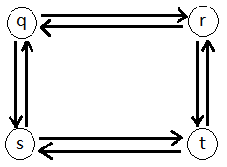
\includegraphics[width=0.25\textwidth]{longestpath.png}
\caption{\label{fig:graph_1}Sample Graph.}
\end{figure}
\vspace{6mm}
\textbf{Overlapping sub-problems} :
\par{\indent Like Divide and Conquer, Dynamic Programming combines solutions to sub-problems. Dynamic Programming is mainly used when solutions of same subproblems are needed again and again. In dynamic programming, computed solutions to subproblems are stored in a table so that these don’t have to be recomputed. So Dynamic Programming is not useful when there are no common (overlapping) subproblems because there is no point storing the solutions if they are not needed again. For example, Binary Search doesn’t have common subproblems. If we take an example of following recursive program for Fibonacci Numbers, there are many subproblems which are solved again and again.
\newline
\begin{lstlisting}
/* simple recursive program for Fibonacci numbers */
int fib(int n) 
{ 
   if ( n <= 1 ) 
      return n; 
   return fib(n-1) + fib(n-2); 
}
\end{lstlisting}
Recursion tree for execution of fib(5)
\begin{figure}[h!]
\centering
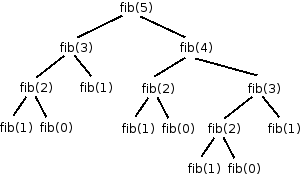
\includegraphics[width=0.5\textwidth]{fib5.png}
\caption{Fibonacci tree}
\end{figure}
We can see that the function fib(3) is being called 2 times. If we would have stored the value of fib(3), then instead of computing it again, we could have reused the old stored value. There are following two different ways to store the values so that these values can be reused:
\begin{enumerate}[label=(\alph*)]
\item Memoization (Top Down)
\item Tabulation (Bottom Up)
\end{enumerate}
So, to use DP, subproblems must be dependent/overlapping. Otherwise, a divide-and-conquer approach is the choice.

\subsection {Tabulation vs Memoization}
\begin{center} \textbf{**Tabulation – Bottom Up Dynamic Programming**} \end{center}
As the name itself suggests starting from the bottom and cumulating answers to the top.Let’s describe a state for our DP problem to be dp[x] with dp[0] as base state and dp[n] as our destination state. So,  we need to find the value of destination state  dp[n].If we start our transition from our base state i.e dp[0] and follow our state transition relation to reach our destination state dp[n], we call it Bottom Up approach as it is quite clear that we started our transition from the bottom base state and reached the top most desired state.
\vspace{3mm}
\begin{lstlisting}
// Bottom up version to find factorial x.
int dp[max];

// base case
int dp[0] = 1;
for (int i = 1; i< =n; i++)
{
    dp[i] = dp[i-1] * i;
}
\end{lstlisting}
The above code clearly follows the bottom-up approach as it starts its transition from the bottom-most base case dp[0] and reaches its destination state dp[n]. Here, we may notice that the dp table is being populated sequentially and we are directly accessing the calculated states from the table itself and hence, we call it tabulation method.
\vspace{3mm}
\begin{center} \textbf{** Memoization Method – Top Down Dynamic Programming**} \end{center}
If we need to find the value for some state say dp[n] and instead of starting from the base state that  dp[0] we ask our answer from the states that can reach the destination state dp[n] following the state transition relation, then it is the top-down fashion of DP. So, we start from dp[n] and to calculate that we go down to dp[n-1] ... ... until we are done calculating and storing dp[0] in this manner. Let's have a look into the code of finding factorial x in this method.
\vspace{3mm}
\begin{lstlisting}
// Top down version to find factorial x.
// To speed up we store the values of calculated states

// initialized to -1
int dp[n]

// return fact x!
int solve(int x)
{
    if (x==0)
        return 1;
    if (dp[x]!=-1)
        return dp[x];
    return (dp[x] = x * solve(x-1));
}
\end{lstlisting}
\vspace{3mm}
As we can see we are storing the most recent solution such a way that if next time we got a call from the same state we simply return it from the memory. So, this is why we call it memoization as we are storing the most recent state values.
\begin{figure}[H]
\centering
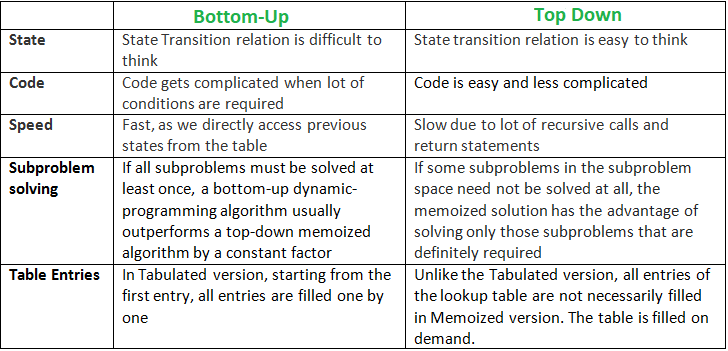
\includegraphics[width=1.0\textwidth]{TabulationvsMemoization.png}
\caption{Comparison between Bottom-up and Top down approach.}
\end{figure}

\section {Examples of Dynamic Programming Problems}
Basic problems -
\begin{enumerate}
\item Fibonacci numbers
\item Tiling Problems
\item Coin change problem
\item Subset sum problem
\item Longest Common Sub-sequence
\item Longest Repeated Subsequence
\item Longest Increasing Subsequence
\item LCS (Longest Common Subsequence) of three strings
\item Warshall’s All pairs shortest path
\item Bellman Ford’s Single Source Shortest Path
\end{enumerate}

Advanced problems - 
\begin{enumerate}
\item Matrix chain multiplication
\item BitMasking
\item Digit DP
\end{enumerate} and so on. Here, we will be discussing about Tiling problem first.

\end{document}